\documentclass[12pt, a4paper]{article}
\usepackage{gset}
\setcounter{MaxMatrixCols}{50}
\begin{document}
	\maintitle{ЛАиГ. Домашнее задание 5}
	\textbf{1. К3.1 (б, в, г)} \bs
	б) $
	\mattwo{\rowsix{1}{2}{3}{4}{5}{6}}{\rowsix{3}{6}{4}{5}{2}{1}} \times \mattwo{\rowsix{1}{2}{3}{4}{5}{6}}{\rowsix{2}{4}{1}{5}{6}{3}} = 
	\mattwo{\rowsix{1}{2}{3}{4}{5}{6}}{\rowsix{6}{5}{3}{2}{1}{4}} \bs 
	\mattwo{\rowsix{1}{2}{3}{4}{5}{6}}{\rowsix{2}{4}{1}{5}{6}{3}} \times
	\mattwo{\rowsix{1}{2}{3}{4}{5}{6}}{\rowsix{3}{6}{4}{5}{2}{1}}  =
	\mattwo{\rowsix{1}{2}{3}{4}{5}{6}}{\rowsix{1}{3}{5}{6}{4}{2}} \bs
	$
	в) $
	\mattwo{\rowfive{1}{2}{3}{4}{5}}{\rowfive{2}{1}{3}{5}{4}} \times
	\mattwo{\rowfive{1}{2}{3}{4}{5}}{\rowfive{4}{5}{3}{2}{1}} = 
	\mattwo{\rowfive{1}{2}{3}{4}{5}}{\rowfive{5}{4}{3}{1}{2}} \bs
	\mattwo{\rowfive{1}{2}{3}{4}{5}}{\rowfive{4}{5}{3}{2}{1}} \times \mattwo{\rowfive{1}{2}{3}{4}{5}}{\rowfive{2}{1}{3}{5}{4}} =
	\mattwo{\rowfive{1}{2}{3}{4}{5}}{\rowfive{5}{4}{3}{1}{2}} \bs
	$
	г) $
	\mattwo{\rowsix{1}{2}{3}{4}{5}{6}}{\rowsix{3}{5}{1}{6}{2}{4}} \times 
	\mattwo{\rowsix{1}{2}{3}{4}{5}{6}}{\rowsix{6}{3}{4}{2}{1}{5}} = 
	\mattwo{\rowsix{1}{2}{3}{4}{5}{6}}{\rowsix{4}{1}{6}{5}{3}{2}} \bs
	$
	\textbf{2. Найдите $\sigma^{2023}$} \bs
	$
	\sigma = \begin{pmatrix} 1 & 2 & 3 & 4 & 5 & 6 & 7 & 8 & 9 & 10 & 11 & 12 \\3 & 4 & 5 & 9 & 12 & 2 & 7 & 1 & 10 & 11 & 6 & 8  \end{pmatrix} \bs
	$
	Найдем циклы в $\sigma$: \sspace
	$\sigma = (1,3,5,12,8) * (2,4,9,10,11,6) * (7)$ \sspace
	$\sigma^{2023} = (1,3,5,12,8)^{2023} * (2,4,9,10,11,6)^{2023} * (7)^{2023} = \sspace = (1,3,5,12,8)^3 * (2,4,9,10,11,6)^1 * (7)^1 = (1, 12, 3, 8, 5) * (2,4,9,10,11,6) * (7) \bs 
	\sigma^{2023} = \begin{pmatrix} 1 & 2 & 3 & 4 & 5 & 6 & 7 & 8 & 9 & 10 & 11 & 12 \\12 & 4 & 8 & 9 & 1 & 2 & 7 & 5 & 10 & 11 & 6 & 3  \end{pmatrix}
	$
	\bs 
	\textbf{3. К3.2 (г, д, е)} \bs
	г) $
	\mattwo{\rowseven{1}{2}{3}{4}{5}{6}{7}}{\rowseven{4}{3}{6}{7}{1}{5}{2}} = (1,4,7,2,3,6,5) \bs
	$
	д) $
	\mattwo{\rowseven{1}{2}{3}{4}{\cdots}{2n-1}{2n}}{\rowseven{2}{1}{4}{3}{\cdots}{2n}{2n-1}} = (1,2) * (3,4)  \cdots (2n-1, 2n) \bs
	$
	е) $
	\mattwo{\roweight{1}{2}{\cdots}{n}{n+1}{n+2}{\cdots}{2n}}{\roweight{n+1}{n+2}{\cdots}{2n}{1}{2}{\cdots}{n}} = (1, n + 1) * (2, n + 2) \cdots (n, 2n) \bs
	$ 
	\textbf{4. К3.5 (б, г, е, ж)} \bs
	б) $
	\sigma = (6, 3, 1, 2, 5, 4) \quad l (\sigma) = 8 \sspace
	$
	г) $
	\sigma = (7, 5, 6, 4, 1, 3, 2) \quad l (\sigma) = 18 \sspace
	$
	е) $
	\sigma = (2,4, 6,..., 2n, 1,3, 5,..., 2n-1) \quad l (\sigma) = 1 + 2 + \cdots + n = \dfrac{n(n + 1)}{2} \sspace
	$
	ж) $
	\sigma = (k,k + 1,...,n,1,2,...,k-1) 
	$
	Так как $1 < 2 < \cdots < k - 1 < k$, то каждый член из первых $n - k + 1$ чисел будет образовывать инверсию с последними $k - 1$ членами последовательности. Поэтому $l(\sigma) = (n - k + 1) * (k - 1)$  \bs
	\textbf{5. Сопряжены ли перестановки $\sigma$ из номера 2 и $\tau$} \sspace
	$\tau =  \begin{pmatrix} 1 & 2 & 3 & 4 & 5 & 6 & 7 & 8 & 9 & 10 & 11 & 12 \\1&3&4&5&11&12&2&9&10&6& 7 & 8  \end{pmatrix}$ \sspace 
	По свойству последовательности сопряжены, если у них совпадает суммарная длина независимых циклов. Найдем суммарные длины циклов $\sigma $ и $\tau$ \sspace
	$\sigma = (1,3,5,12,8) * (2,4,9,10,11,6) * (7) \quad S = \{1, 5, 6\}$  \sspace
	$\tau = (1) * (2, 3,4,5,11,7) * (6,12,8,9,10)  \quad S = \{1, 5, 6\}$ \sspace
	Так как множества длин независимых циклов совпадают, то последовательности сопряжены (доказывали на семинаре). \newpage
	\textbf{6. Докажите, что любую транспозицию можно представить в виде произведения нечётного числа элементарных транспозиций} \bs
	Пусть в перестановке транспозиция меняет элементы i, j. Тогда можно осуществить эту транспозицию по такому алгоритму. Сначала переставить $i$ элемент в $j$ место, сдвигая все элементы кроме $i$ влево на 1 место за $(j - i)$ элементарных перестановок. Затем передвинуть $j$ элемент на $i$ место за $(j - i - 1)$ элементарных перестановок. Итого элементарных перестановок $2(j - i) - 1$, что является нечетным числом \sspace
	\[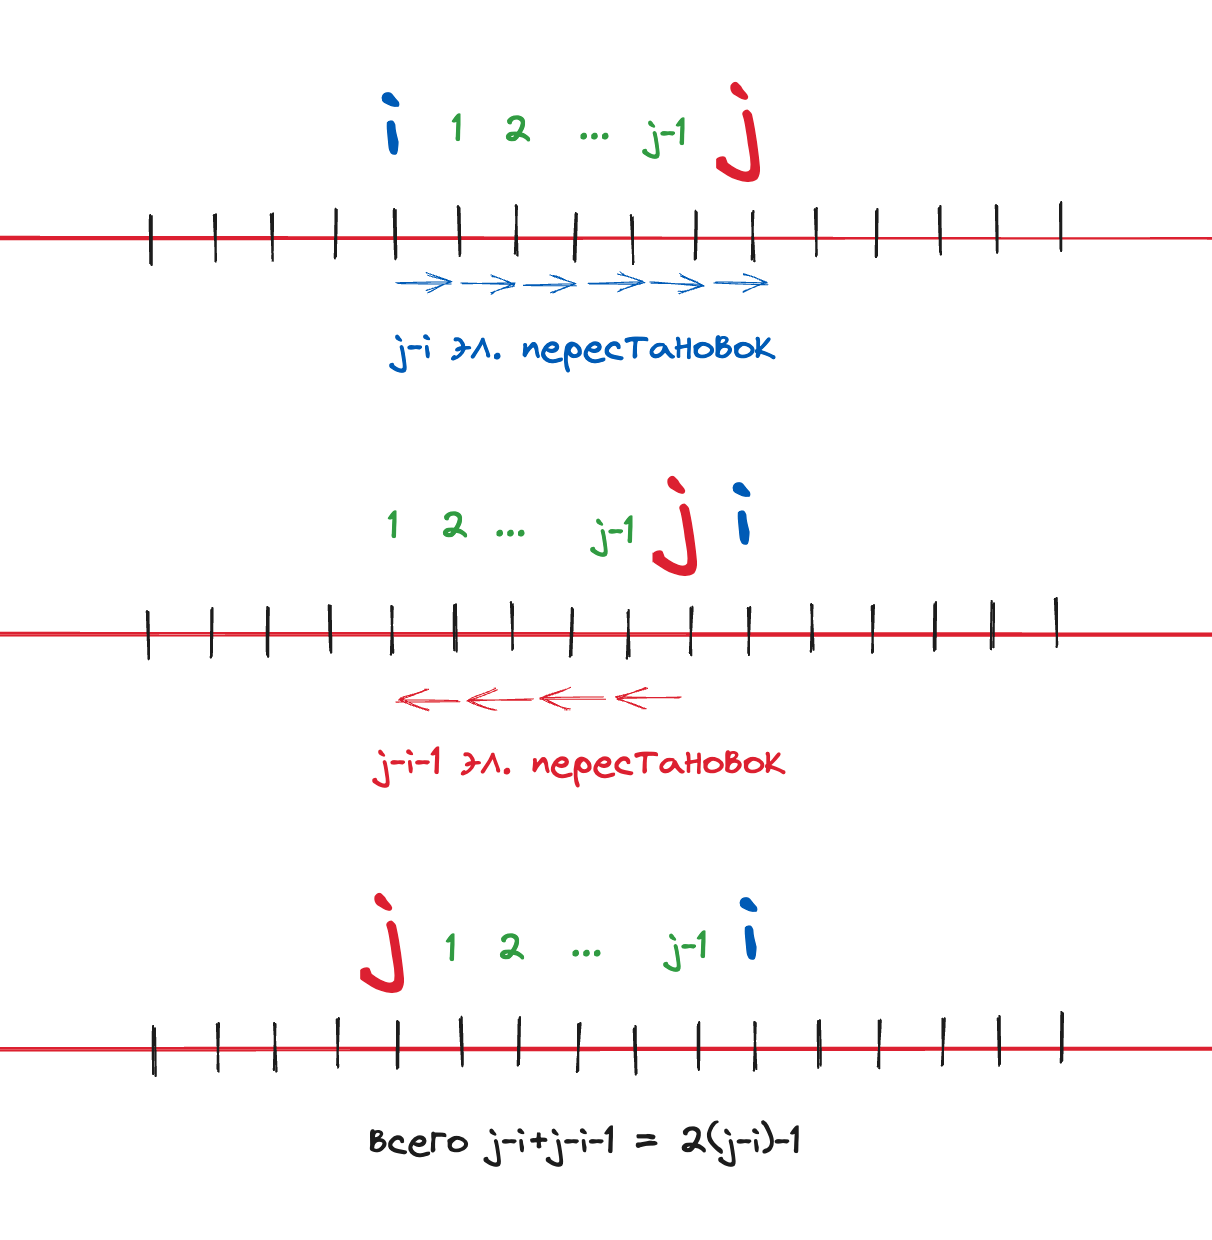
\includegraphics[width=125mm]{img1}\] \bs
	\textbf{7) К3.8} \bs
	Рассмотрим $a_x = i$, всего чисел от 1 до n меньших $i$ ровно $i - 1$. Пусть $m$ из них образовывали инверсию с $a_x$ в первой перестановке. Тогда оставшиеся $i - 1 - m$ чисел стояли "слева" \space от $a_x$. Тогда во второй перестановке эти числа будут стоять "справа" \space от $a_x$, а значит образовывать с этим элементом инверсию. Итого в двух перестановках для $a_x = i$ образовывается $m + i - 1 - m = i - 1$ инверсий. Значит всего в двух перестановках $1 + 2 + \cdots + n - 1 = \dfrac{n(n - 1)}{2}$ инверсий. Следовательно во второй перестановке  $\dfrac{n(n - 1)}{2} - k$ инверсий.
\end{document}